\documentclass[]{report}
\usepackage{lmodern}
\usepackage{amssymb,amsmath}
\usepackage{ifxetex,ifluatex}
\usepackage{fixltx2e} % provides \textsubscript
\ifnum 0\ifxetex 1\fi\ifluatex 1\fi=0 % if pdftex
  \usepackage[T1]{fontenc}
  \usepackage[utf8]{inputenc}
\else % if luatex or xelatex
  \ifxetex
    \usepackage{mathspec}
  \else
    \usepackage{fontspec}
  \fi
  \defaultfontfeatures{Ligatures=TeX,Scale=MatchLowercase}
\fi
% use upquote if available, for straight quotes in verbatim environments
\IfFileExists{upquote.sty}{\usepackage{upquote}}{}
% use microtype if available
\IfFileExists{microtype.sty}{%
\usepackage{microtype}
\UseMicrotypeSet[protrusion]{basicmath} % disable protrusion for tt fonts
}{}
\usepackage{hyperref}
\hypersetup{unicode=true,
            pdftitle={Data 624 - Group 2 Homework Part 2},
            pdfauthor={Vinicio Haro; Sang Yoon (Andy) Hwang; Julian McEachern; Jeremy O'Brien; Bethany Poulin},
            pdfborder={0 0 0},
            breaklinks=true}
\urlstyle{same}  % don't use monospace font for urls
\usepackage{color}
\usepackage{fancyvrb}
\newcommand{\VerbBar}{|}
\newcommand{\VERB}{\Verb[commandchars=\\\{\}]}
\DefineVerbatimEnvironment{Highlighting}{Verbatim}{commandchars=\\\{\}}
% Add ',fontsize=\small' for more characters per line
\usepackage{framed}
\definecolor{shadecolor}{RGB}{248,248,248}
\newenvironment{Shaded}{\begin{snugshade}}{\end{snugshade}}
\newcommand{\AlertTok}[1]{\textcolor[rgb]{0.94,0.16,0.16}{#1}}
\newcommand{\AnnotationTok}[1]{\textcolor[rgb]{0.56,0.35,0.01}{\textbf{\textit{#1}}}}
\newcommand{\AttributeTok}[1]{\textcolor[rgb]{0.77,0.63,0.00}{#1}}
\newcommand{\BaseNTok}[1]{\textcolor[rgb]{0.00,0.00,0.81}{#1}}
\newcommand{\BuiltInTok}[1]{#1}
\newcommand{\CharTok}[1]{\textcolor[rgb]{0.31,0.60,0.02}{#1}}
\newcommand{\CommentTok}[1]{\textcolor[rgb]{0.56,0.35,0.01}{\textit{#1}}}
\newcommand{\CommentVarTok}[1]{\textcolor[rgb]{0.56,0.35,0.01}{\textbf{\textit{#1}}}}
\newcommand{\ConstantTok}[1]{\textcolor[rgb]{0.00,0.00,0.00}{#1}}
\newcommand{\ControlFlowTok}[1]{\textcolor[rgb]{0.13,0.29,0.53}{\textbf{#1}}}
\newcommand{\DataTypeTok}[1]{\textcolor[rgb]{0.13,0.29,0.53}{#1}}
\newcommand{\DecValTok}[1]{\textcolor[rgb]{0.00,0.00,0.81}{#1}}
\newcommand{\DocumentationTok}[1]{\textcolor[rgb]{0.56,0.35,0.01}{\textbf{\textit{#1}}}}
\newcommand{\ErrorTok}[1]{\textcolor[rgb]{0.64,0.00,0.00}{\textbf{#1}}}
\newcommand{\ExtensionTok}[1]{#1}
\newcommand{\FloatTok}[1]{\textcolor[rgb]{0.00,0.00,0.81}{#1}}
\newcommand{\FunctionTok}[1]{\textcolor[rgb]{0.00,0.00,0.00}{#1}}
\newcommand{\ImportTok}[1]{#1}
\newcommand{\InformationTok}[1]{\textcolor[rgb]{0.56,0.35,0.01}{\textbf{\textit{#1}}}}
\newcommand{\KeywordTok}[1]{\textcolor[rgb]{0.13,0.29,0.53}{\textbf{#1}}}
\newcommand{\NormalTok}[1]{#1}
\newcommand{\OperatorTok}[1]{\textcolor[rgb]{0.81,0.36,0.00}{\textbf{#1}}}
\newcommand{\OtherTok}[1]{\textcolor[rgb]{0.56,0.35,0.01}{#1}}
\newcommand{\PreprocessorTok}[1]{\textcolor[rgb]{0.56,0.35,0.01}{\textit{#1}}}
\newcommand{\RegionMarkerTok}[1]{#1}
\newcommand{\SpecialCharTok}[1]{\textcolor[rgb]{0.00,0.00,0.00}{#1}}
\newcommand{\SpecialStringTok}[1]{\textcolor[rgb]{0.31,0.60,0.02}{#1}}
\newcommand{\StringTok}[1]{\textcolor[rgb]{0.31,0.60,0.02}{#1}}
\newcommand{\VariableTok}[1]{\textcolor[rgb]{0.00,0.00,0.00}{#1}}
\newcommand{\VerbatimStringTok}[1]{\textcolor[rgb]{0.31,0.60,0.02}{#1}}
\newcommand{\WarningTok}[1]{\textcolor[rgb]{0.56,0.35,0.01}{\textbf{\textit{#1}}}}
\usepackage{graphicx,grffile}
\makeatletter
\def\maxwidth{\ifdim\Gin@nat@width>\linewidth\linewidth\else\Gin@nat@width\fi}
\def\maxheight{\ifdim\Gin@nat@height>\textheight\textheight\else\Gin@nat@height\fi}
\makeatother
% Scale images if necessary, so that they will not overflow the page
% margins by default, and it is still possible to overwrite the defaults
% using explicit options in \includegraphics[width, height, ...]{}
\setkeys{Gin}{width=\maxwidth,height=\maxheight,keepaspectratio}
\IfFileExists{parskip.sty}{%
\usepackage{parskip}
}{% else
\setlength{\parindent}{0pt}
\setlength{\parskip}{6pt plus 2pt minus 1pt}
}
\setlength{\emergencystretch}{3em}  % prevent overfull lines
\providecommand{\tightlist}{%
  \setlength{\itemsep}{0pt}\setlength{\parskip}{0pt}}
\setcounter{secnumdepth}{0}

%%% Use protect on footnotes to avoid problems with footnotes in titles
\let\rmarkdownfootnote\footnote%
\def\footnote{\protect\rmarkdownfootnote}

%%% Change title format to be more compact
\usepackage{titling}

% Create subtitle command for use in maketitle
\providecommand{\subtitle}[1]{
  \posttitle{
    \begin{center}\large#1\end{center}
    }
}

\setlength{\droptitle}{-2em}

  \title{Data 624 - Group 2\\
Homework Part 2}
    \pretitle{\vspace{\droptitle}\centering\huge}
  \posttitle{\par}
    \author{Vinicio Haro \\ Sang Yoon (Andy) Hwang \\ Julian McEachern \\ Jeremy O'Brien \\ Bethany Poulin}
    \preauthor{\centering\large\emph}
  \postauthor{\par}
      \predate{\centering\large\emph}
  \postdate{\par}
    \date{16 December 2019}

% set plain style for page numbers
\pagestyle{plain}
\raggedbottom

% change font
\usepackage{fontspec}
\setmainfont{Arial}

% create color block quotes
\usepackage[dvipsnames]{xcolor}
\usepackage{tcolorbox}     
\newtcolorbox{question}[1]{colback=white, colframe=Emerald ,fonttitle=\bfseries, title=#1}

\newtcolorbox{subquestion}[1]{colback=white,colframe=white, coltitle=Emerald!75!black, detach title, before upper={\tcbtitle\quad\hangindent7mm}, title={#1},fonttitle=\bfseries, fontupper=\bfseries}

% remove "chapter" from chapter title
\usepackage{titlesec}

\titleformat{\chapter}
  {\normalfont\LARGE\bfseries}{\thechapter}{1em}{}
\titlespacing*{\chapter}{0pt}{3.5ex plus 1ex minus .2ex}{2.3ex plus .2ex}

\usepackage{titling}
\pretitle{\begin{flushright}\LARGE}
\posttitle{\par\end{flushright}\vskip 0.5em}
\preauthor{\begin{flushright}\large \lineskip 0.5em}
\postauthor{\par\end{flushright}}
\predate{\begin{flushright}\large}
\postdate{\par\end{flushright}}


% wrap text
\usepackage{geometry}[textwidth=6in]

% kable 
\usepackage{tabu}
\usepackage{float} 

% multicolumn
\usepackage{multicol}
\usepackage{booktabs}
\usepackage{longtable}
\usepackage{array}
\usepackage{multirow}
\usepackage{wrapfig}
\usepackage{float}
\usepackage{colortbl}
\usepackage{pdflscape}
\usepackage{tabu}
\usepackage{threeparttable}
\usepackage{threeparttablex}
\usepackage[normalem]{ulem}
\usepackage{makecell}
\usepackage{xcolor}

\begin{document}
\maketitle

{
\setcounter{tocdepth}{2}
\tableofcontents
}
\hypertarget{Overview}{%
\chapter*{Getting Started}\label{Overview}}
\addcontentsline{toc}{chapter}{Getting Started}

\hypertarget{overview}{%
\section{Overview}\label{overview}}

Include details on our process in creating this document.

\hypertarget{dependencies}{%
\section{Dependencies}\label{dependencies}}

\begin{Shaded}
\begin{Highlighting}[]
\CommentTok{# Predictive Modeling}
\KeywordTok{libraries}\NormalTok{(}\StringTok{"AppliedPredictiveModeling"}\NormalTok{, }\StringTok{"mlbench"}\NormalTok{, }\StringTok{"caret"}\NormalTok{, }
    \StringTok{"randomForest"}\NormalTok{)}

\CommentTok{# Formatting Libraries}
\KeywordTok{libraries}\NormalTok{(}\StringTok{"default"}\NormalTok{, }\StringTok{"knitr"}\NormalTok{, }\StringTok{"kableExtra"}\NormalTok{)}

\CommentTok{# Plotting Libraries}
\KeywordTok{libraries}\NormalTok{(}\StringTok{"ggplot2"}\NormalTok{, }\StringTok{"grid"}\NormalTok{, }\StringTok{"ggfortify"}\NormalTok{)}
\end{Highlighting}
\end{Shaded}

\newpage

\hypertarget{AS-1}{%
\chapter*{Assignment 1}\label{AS-1}}
\addcontentsline{toc}{chapter}{Assignment 1}

\addcontentsline{toc}{subsection}{Kuhn and Johnson 6.3}

\begin{question}{Kuhn and Johnson 6.3}A chemical manufacturing process for a pharmaceutical product was discussed in Sect.1.4. In this problem, the objective is to understand the relationship between biological measurements of the raw materials (predictors), measurements of the manufacturing process (predictors), and the response of product yield. Biological predictors cannot be changed but can be used to assess the quality of the raw material before processing. On the other hand, manufacturing process predictors can be changed in the manufacturing process. Improving product yield by 1\% will boost revenue by approximately one hundred thousand dollars per batch:\end{question}

\begin{subquestion}{(a).}Start R and use these commands to load the data:
\end{subquestion}

\begin{Shaded}
\begin{Highlighting}[]
\KeywordTok{data}\NormalTok{(}\StringTok{"ChemicalManufacturingProcess"}\NormalTok{)}
\end{Highlighting}
\end{Shaded}

\begin{subquestion}{(b).} A small percentage of cells in the predictor set contain missing values. Use an imputation function to fill in these missing values (e.g., see Sect. 3.8). 
\end{subquestion}

\begin{subquestion}{(c).} Split the data into a training and a test set, pre-process the data, and tune a model of your choice from this chapter. What is the optimal value of the performance metric? 
\end{subquestion}

\begin{subquestion}{(d).} Predict the response for the test set. What is the value of the performance metric and how does this compare with the resampled performance metric on the training set? 
\end{subquestion}

\begin{subquestion}{(e).} Which predictors are most important in the model you have trained? Do either the biological or process predictors dominate the list? 
\end{subquestion}

\begin{subquestion}{(f).} Explore the relationships between each of the top predictors and the response. How could this information be helpful in improving yield in future runs of the manufacturing process?
\end{subquestion}

\hypertarget{AS-2}{%
\chapter*{Assignment 2}\label{AS-2}}
\addcontentsline{toc}{chapter}{Assignment 2}

\addcontentsline{toc}{subsection}{Kuhn and Johnson 7.2}

\begin{question}{Kuhn and Johnson 7.2}Friedman (1991) introduced several benchmark data sets create by simulation. One of these simulations used the following nonlinear equation to create data: $y = 10\text{sin}(\pi x_1 x_2)+20(x_3-0.5)^2+10x_4+5x_5+N(0\text{,} \sigma^2)$; where the $x$ values are random variables uniformly distributed between $[0, 1]$ (there are also 5 other non-informative variables also created in the simulation). \end{question}

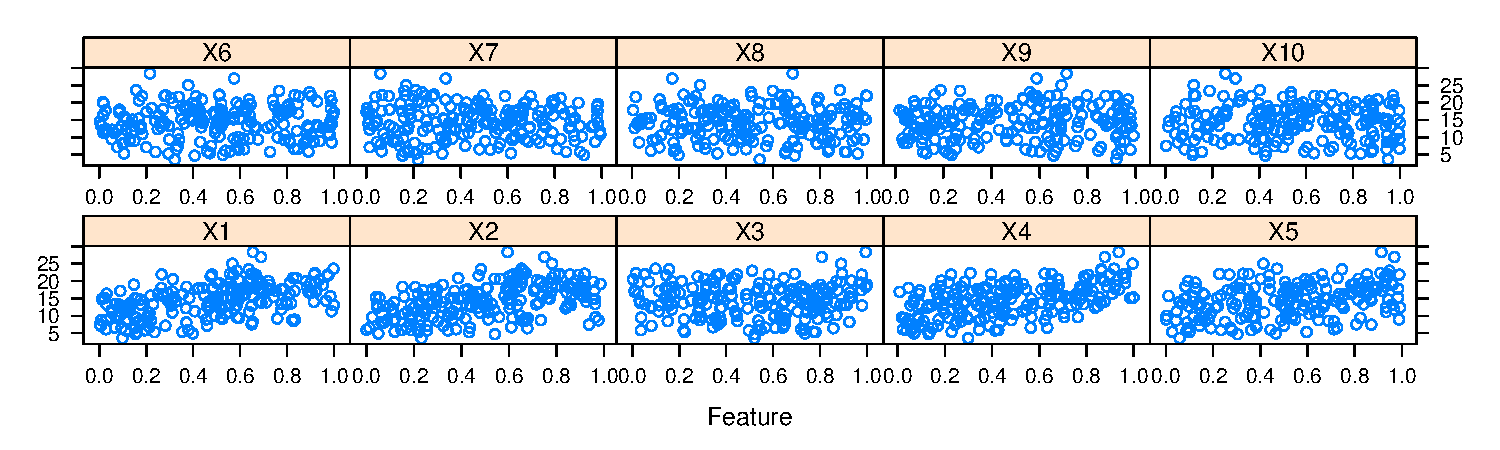
\includegraphics{Homework-Two_files/figure-latex/kj-7.2-ex1-1.pdf}

\begin{subquestion}{(a).} Tune several models on these data. For example: 
\end{subquestion}

Model 1:

Model 2:

Model 3:

\begin{subquestion}{(b).}
Which models appear to give the best performance? Does MARS select the informative predictors (those named X1-X5)?
\end{subquestion}

\addcontentsline{toc}{subsection}{Kuhn and Johnson 7.5}

\begin{question}{Kuhn and Johnson 7.5}
Exercise 6.3 describes data for a chemical manufacturing process. Use the same data imputation, data splitting, and pre-processing steps as before and train several nonlinear regression models.
\end{question}

\begin{subquestion}{(a).}
Which nonlinear regression model gives the optimal resampling and test set performance? 
\end{subquestion}

\begin{subquestion}{(b).}
Which predictors are most important in the optimal nonlinear regression model? Do either the biological or process variables dominate the list? How do the top ten important predictors compare to the top ten predictors from the optimal linear model? 
\end{subquestion}

\begin{subquestion}{(c).}
Explore the relationships between the top predictors and the response for the predictors that are unique to the optimal nonlinear regression model. Do these plots reveal intuition about the biological or process predictors and their relationship with yield?
\end{subquestion}

\hypertarget{AS-3}{%
\chapter*{Assignment 3}\label{AS-3}}
\addcontentsline{toc}{chapter}{Assignment 3}

\addcontentsline{toc}{subsection}{Kuhn and Johnson 8.1}

\begin{question}{Kuhn and Johnson 8.1} Recreate the simulated data from Exercise 7.2: \end{question}

\begin{subquestion}{(a).} Fit a random forest model to all of the predictors, then estimate the variable importance scores. Did the random forest model significantly use the uninformative predictors (V6-V10)?\end{subquestion}

\begin{subquestion}{(b).} Now add an additional predictor that is highly correlated with one of the informative predictors. Fit another random forest model to these data. Did the importance score for V1 change? What happens when you add another predictor that is also highly correlated with V1? For example:\end{subquestion}

\begin{subquestion}{(c).} Use the `cforest` function in the party package to fit a random forest model using conditional inference trees. The party package function `varimp` can calculate predictor importance. The `conditional` argument of that function toggles between the traditional importance measure and the modified version described in Strobl et al. (2007). Do these importances show the same pattern as the traditional random forest model?\end{subquestion}

\begin{subquestion}{(d).} Repeat this process with different tree models, such as boosted trees and Cubist. Does the same pattern occur?\end{subquestion}

\addcontentsline{toc}{subsection}{Kuhn and Johnson 8.2}

\begin{question}{Kuhn and Johnson 8.2}Use a simulation to show tree bias with different granularities.\end{question}

\addcontentsline{toc}{subsection}{Kuhn and Johnson 8.3}

\begin{question}{Kuhn and Johnson 8.3} In stochastic gradient boosting the bagging fraction and learning rate will govern the construction of the trees as they are guided by the gradient. Although the optimal values of these parameters should be obtained through the tuning process, it is helpful to understand how the magnitudes of these parameters affect magnitudes of variable importance. Figure 8.24 provides the variable importance plots for boosting using two extreme values for the bagging fraction (0.1 and 0.9) and the learning rate (0.1 and 0.9) for the solubility data. The left-hand plot has both parameters set to 0.1, and the right-hand plot has both set to 0.9: \end{question}

\begin{subquestion}{(a).} Why does the model on the right focus its importance on just the first few of predictors, whereas the model on the left spreads importance across more predictors? \end{subquestion}

\begin{subquestion}{(b).} Which model do you think would be more predictive of other samples?\end{subquestion}

\begin{subquestion}{(c).} How would increasing interaction depth affect the slope of predictor importance for either model in Fig.8.24?\end{subquestion}

\addcontentsline{toc}{subsection}{Kuhn and Johnson 8.7}

\begin{question}{Kuhn and Johnson 8.7}
Refer to Exercises 6.3 and 7.5 which describe a chemical manufacturing process. Use the same data imputation, data splitting, and pre-processing steps as before and train several tree-based models:
\end{question}

\begin{subquestion}{(a).} Which tree-based regression model gives the optimal resampling and test set performance? \end{subquestion}

\begin{subquestion}{(b).} Which predictors are most important in the optimal tree-based regression model? Do either the biological or process variables dominate the list? How do the top 10 important predictors compare to the top 10 predictors from the optimal linear and nonlinear models?\end{subquestion}

\begin{subquestion}{(c).} Plot the optimal single tree with the distribution of yield in the terminal nodes. Does this view of the data provide additional knowledge about the biological or process predictors and their relationship with yield?\end{subquestion}

\hypertarget{AS-4}{%
\chapter*{Assignment 4}\label{AS-4}}
\addcontentsline{toc}{chapter}{Assignment 4}

\hypertarget{tbd}{%
\section{TBD}\label{tbd}}

\hypertarget{R-Script}{%
\chapter*{R Script}\label{R-Script}}
\addcontentsline{toc}{chapter}{R Script}


\end{document}
